\documentclass{beamer}\usepackage{graphicx, color}
%% maxwidth is the original width if it is less than linewidth
%% otherwise use linewidth (to make sure the graphics do not exceed the margin)
\makeatletter
\def\maxwidth{ %
  \ifdim\Gin@nat@width>\linewidth
    \linewidth
  \else
    \Gin@nat@width
  \fi
}
\makeatother

\IfFileExists{upquote.sty}{\usepackage{upquote}}{}
\definecolor{fgcolor}{rgb}{0.2, 0.2, 0.2}
\newcommand{\hlnumber}[1]{\textcolor[rgb]{0,0,0}{#1}}%
\newcommand{\hlfunctioncall}[1]{\textcolor[rgb]{0.501960784313725,0,0.329411764705882}{\textbf{#1}}}%
\newcommand{\hlstring}[1]{\textcolor[rgb]{0.6,0.6,1}{#1}}%
\newcommand{\hlkeyword}[1]{\textcolor[rgb]{0,0,0}{\textbf{#1}}}%
\newcommand{\hlargument}[1]{\textcolor[rgb]{0.690196078431373,0.250980392156863,0.0196078431372549}{#1}}%
\newcommand{\hlcomment}[1]{\textcolor[rgb]{0.180392156862745,0.6,0.341176470588235}{#1}}%
\newcommand{\hlroxygencomment}[1]{\textcolor[rgb]{0.43921568627451,0.47843137254902,0.701960784313725}{#1}}%
\newcommand{\hlformalargs}[1]{\textcolor[rgb]{0.690196078431373,0.250980392156863,0.0196078431372549}{#1}}%
\newcommand{\hleqformalargs}[1]{\textcolor[rgb]{0.690196078431373,0.250980392156863,0.0196078431372549}{#1}}%
\newcommand{\hlassignement}[1]{\textcolor[rgb]{0,0,0}{\textbf{#1}}}%
\newcommand{\hlpackage}[1]{\textcolor[rgb]{0.588235294117647,0.709803921568627,0.145098039215686}{#1}}%
\newcommand{\hlslot}[1]{\textit{#1}}%
\newcommand{\hlsymbol}[1]{\textcolor[rgb]{0,0,0}{#1}}%
\newcommand{\hlprompt}[1]{\textcolor[rgb]{0.2,0.2,0.2}{#1}}%

\usepackage{framed}
\makeatletter
\newenvironment{kframe}{%
 \def\at@end@of@kframe{}%
 \ifinner\ifhmode%
  \def\at@end@of@kframe{\end{minipage}}%
  \begin{minipage}{\columnwidth}%
 \fi\fi%
 \def\FrameCommand##1{\hskip\@totalleftmargin \hskip-\fboxsep
 \colorbox{shadecolor}{##1}\hskip-\fboxsep
     % There is no \\@totalrightmargin, so:
     \hskip-\linewidth \hskip-\@totalleftmargin \hskip\columnwidth}%
 \MakeFramed {\advance\hsize-\width
   \@totalleftmargin\z@ \linewidth\hsize
   \@setminipage}}%
 {\par\unskip\endMakeFramed%
 \at@end@of@kframe}
\makeatother

\definecolor{shadecolor}{rgb}{.97, .97, .97}
\definecolor{messagecolor}{rgb}{0, 0, 0}
\definecolor{warningcolor}{rgb}{1, 0, 1}
\definecolor{errorcolor}{rgb}{1, 0, 0}
\newenvironment{knitrout}{}{} % an empty environment to be redefined in TeX

\usepackage{alltt}
\usepackage{graphicx, parskip, microtype, hyperref}

\frenchspacing

\usetheme{default}
\usecolortheme{orchid}




\title{ggplot2: visualizing our data and IO}
\author{Peter D Smits}
\institute{Committee on Evolutionary Biology \\
University of Chicago}
\date{\today}

\begin{document}

\begin{frame}
  \maketitle
\end{frame}

\begin{frame}
  \frametitle{Introduction}

  Last time, we covered the basics of ggplot2 and how we modify plots.

  Today's talk will be in two parts. 
  \begin{enumerate}
    \item introduction to maps and ggplot
    \item Sample workflow from IO through munging to visualizing.
  \end{enumerate}

\end{frame}

\begin{frame}[fragile]
  \frametitle{Maps}
\begin{knitrout}\scriptsize
\definecolor{shadecolor}{rgb}{0.969, 0.969, 0.969}\color{fgcolor}\begin{kframe}
\begin{alltt}
\hlfunctioncall{require}(ggplot2)
\hlfunctioncall{library}(maps)
nz <- \hlfunctioncall{map_data}(\hlstring{'nz'})
\end{alltt}
\end{kframe}
\end{knitrout}


% latex table generated in R 2.15.2 by xtable 1.7-0 package
% Thu Jan 24 18:55:41 2013
\begin{table}[ht]
\begin{center}
\begin{tabular}{rrrrrll}
  \hline
 & long & lat & group & order & region & subregion \\ 
  \hline
1 & 172.74 & -34.44 & 1.00 &   1 & North.Island  &  \\ 
  2 & 172.80 & -34.46 & 1.00 &   2 & North.Island  &  \\ 
  3 & 172.85 & -34.45 & 1.00 &   3 & North.Island  &  \\ 
  4 & 172.90 & -34.42 & 1.00 &   4 & North.Island  &  \\ 
  5 & 172.96 & -34.43 & 1.00 &   5 & North.Island  &  \\ 
  6 & 173.02 & -34.40 & 1.00 &   6 & North.Island  &  \\ 
   \hline
\end{tabular}
\end{center}
\end{table}



\end{frame}

\begin{frame}[fragile]
  \frametitle{Looking at NZ: Cartesian coordinates}
\begin{knitrout}\scriptsize
\definecolor{shadecolor}{rgb}{0.969, 0.969, 0.969}\color{fgcolor}\begin{kframe}
\begin{alltt}
nzmap <- \hlfunctioncall{ggplot}(nz, \hlfunctioncall{aes}(x = long, y = lat, group = group))
nzmap <- nzmap + \hlfunctioncall{geom_polygon}(fill = \hlstring{'white'}, colour = \hlstring{'black'})
nzmap
\end{alltt}
\end{kframe}
\end{knitrout}

\end{frame}

\begin{frame}[fragile]
\begin{knitrout}\scriptsize
\definecolor{shadecolor}{rgb}{0.969, 0.969, 0.969}\color{fgcolor}
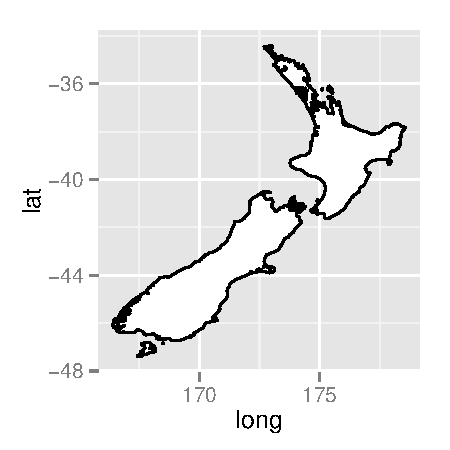
\includegraphics[width=\maxwidth]{figure/unnamed-chunk-5} 

\end{knitrout}

\end{frame}

\begin{frame}[fragile]
  \frametitle{Looking at NZ: Mercator projection}
  \begin{columns}
    \begin{column}{0.3\textwidth}
\begin{knitrout}\scriptsize
\definecolor{shadecolor}{rgb}{0.969, 0.969, 0.969}\color{fgcolor}\begin{kframe}
\begin{alltt}
\hlfunctioncall{library}(mapproj)
nzmap + \hlfunctioncall{coord_map}()
\end{alltt}
\end{kframe}
\end{knitrout}

    \end{column}
    \begin{column}{0.7\textwidth}
\begin{knitrout}\scriptsize
\definecolor{shadecolor}{rgb}{0.969, 0.969, 0.969}\color{fgcolor}
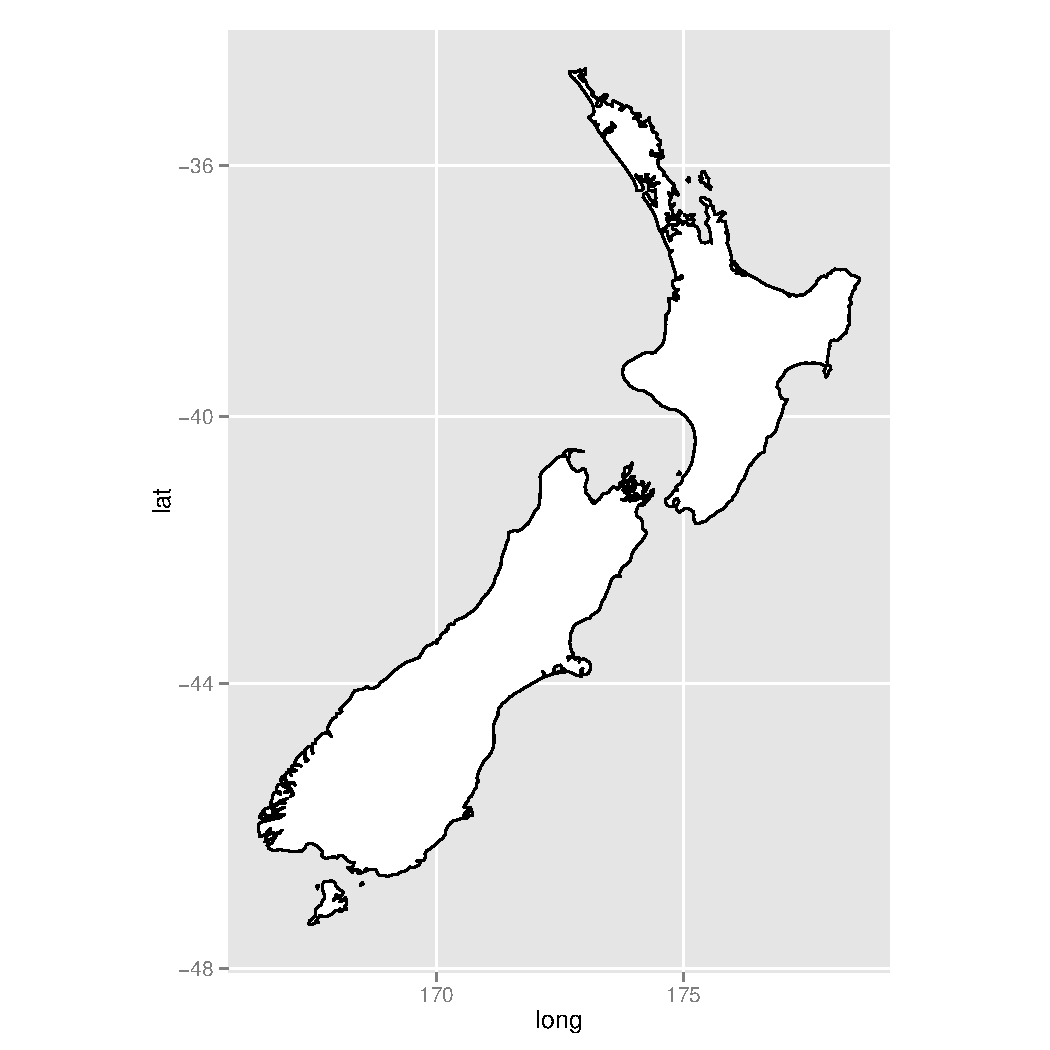
\includegraphics[width=\maxwidth]{figure/unnamed-chunk-7} 

\end{knitrout}

    \end{column}
  \end{columns}
\end{frame}

\begin{frame}[fragile]
  \frametitle{Looking NZ: Other projections}
\begin{knitrout}\scriptsize
\definecolor{shadecolor}{rgb}{0.969, 0.969, 0.969}\color{fgcolor}\begin{kframe}
\begin{alltt}
nzmap + \hlfunctioncall{coord_map}(\hlstring{'cylindrical'})

nzmap + \hlfunctioncall{coord_map}(\hlstring{'azequalarea'}, 
                  orientation = \hlfunctioncall{c}(-36.92, 174.6, 0))

\hlcomment{## ?mapproject for coordinate systems and their parameters}
\hlcomment{## there are a lot of them}
\end{alltt}
\end{kframe}
\end{knitrout}

\end{frame}

\begin{frame}[fragile]
  \frametitle{World map!}
\begin{knitrout}\scriptsize
\definecolor{shadecolor}{rgb}{0.969, 0.969, 0.969}\color{fgcolor}\begin{kframe}
\begin{alltt}
world <- \hlfunctioncall{map_data}(\hlstring{'world'})
worldmap <- \hlfunctioncall{ggplot}(world, \hlfunctioncall{aes}(x = long, y = lat, group = group))
worldmap <- worldmap + \hlfunctioncall{geom_path}()
worldmap <- worldmap + \hlfunctioncall{scale_y_continuous}(breaks = (-2:2) * 30) + 
            \hlfunctioncall{scale_x_continuous}(breaks = (-4:4) * 45)
worldmap <- worldmap + \hlfunctioncall{coord_equal}()
\end{alltt}
\end{kframe}
\end{knitrout}

\end{frame}

\begin{frame}[fragile]
\begin{knitrout}\scriptsize
\definecolor{shadecolor}{rgb}{0.969, 0.969, 0.969}\color{fgcolor}
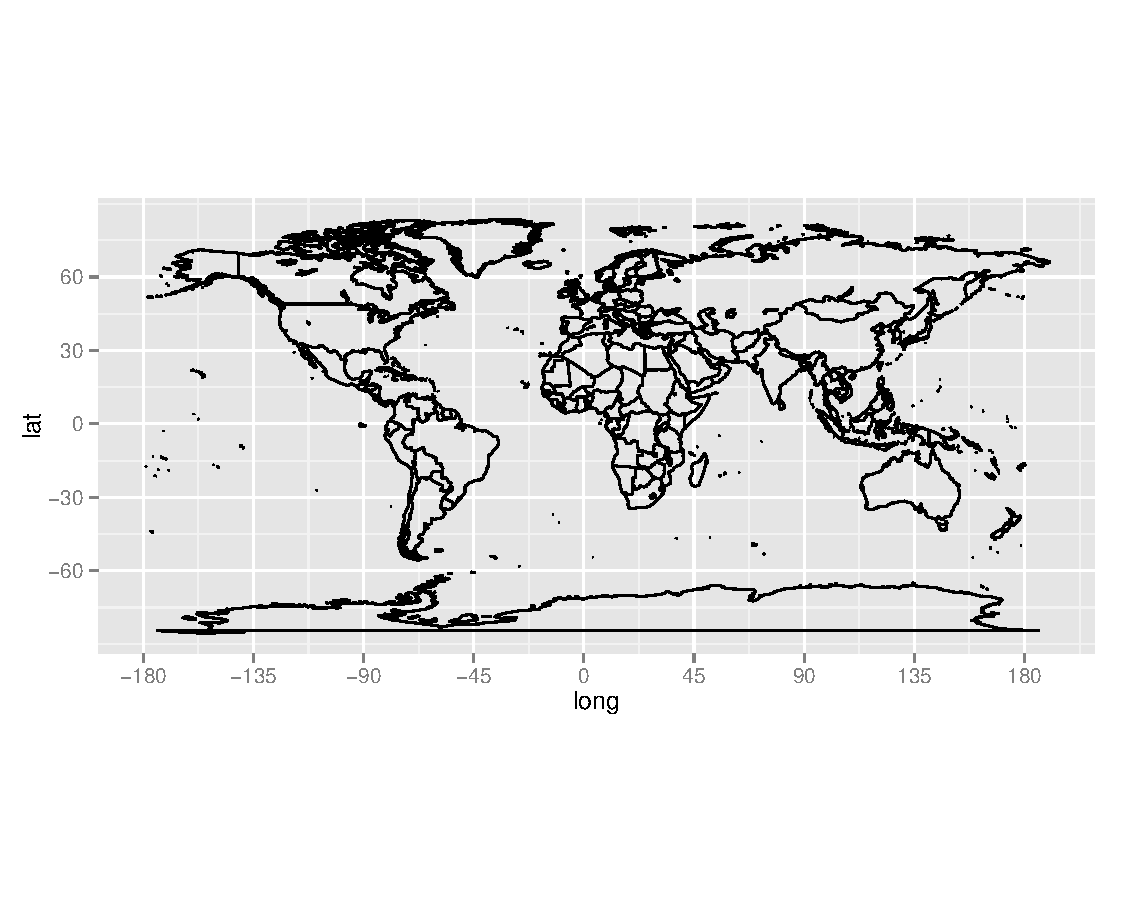
\includegraphics[width=\maxwidth]{figure/unnamed-chunk-10} 

\end{knitrout}

\end{frame}

\begin{frame}[fragile]
  \frametitle{Lets add random dots to it!}
\begin{knitrout}\scriptsize
\definecolor{shadecolor}{rgb}{0.969, 0.969, 0.969}\color{fgcolor}\begin{kframe}
\begin{alltt}
x.long <- \hlfunctioncall{rnorm}(100, mean = \hlfunctioncall{mean}(world$long), sd = \hlfunctioncall{sd}(world$long))
y.lat <- \hlfunctioncall{rnorm}(100, mean = \hlfunctioncall{mean}(world$lat), sd = \hlfunctioncall{sd}(world$lat))
rpoints <- \hlfunctioncall{data.frame}(x.long, y.lat)
\hlcomment{## there are prettier ways to do this, but they are more complicated}
worldmap <- worldmap + \hlfunctioncall{geom_point}(data = rpoints,
                                  mapping = \hlfunctioncall{aes}(x = x.long, 
                                                y = y.lat, 
                                                group = NULL),
                                  colour = \hlstring{'red'})
worldmap <- worldmap + \hlfunctioncall{theme_minimal}()
\end{alltt}
\end{kframe}
\end{knitrout}

\end{frame}

\begin{frame}
\begin{knitrout}\scriptsize
\definecolor{shadecolor}{rgb}{0.969, 0.969, 0.969}\color{fgcolor}
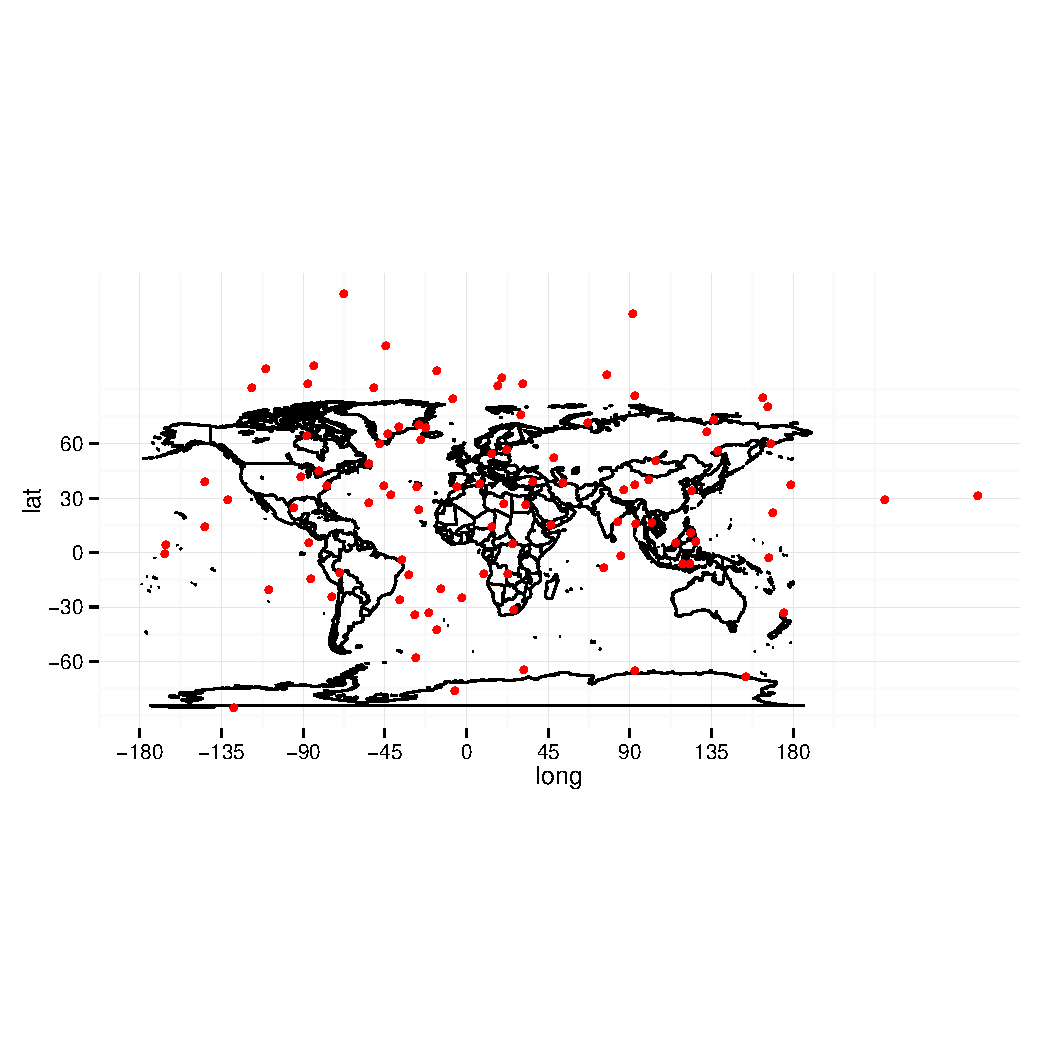
\includegraphics[width=\maxwidth]{figure/unnamed-chunk-12} 

\end{knitrout}

\end{frame}

\begin{frame}
  \frametitle{More on maps}

  Try a lot of projections to get the one that distorts your reality the least.

  You can cut down the amount of the map displayed. You can look that up on your own.

  Shape files can be read into R and used as maps. (maptools)

  There are packages to use google maps. (RGoogleMaps, ggmap)

\end{frame}

\begin{frame}[fragile]
  \frametitle{IO}

  Input/Output: the act of getting things in and out or your program/script/what have you.

\begin{knitrout}\scriptsize
\definecolor{shadecolor}{rgb}{0.969, 0.969, 0.969}\color{fgcolor}\begin{kframe}
\begin{alltt}
\hlfunctioncall{read.table}()
\hlfunctioncall{read.csv}()
\hlfunctioncall{read.tree}()
\hlfunctioncall{read.nexus}()
\hlfunctioncall{dget}()
\hlcomment{## etc.}

\hlfunctioncall{write.table}()
\hlfunctioncall{write.csv}()
\hlfunctioncall{write.tree}()
\hlfunctioncall{write.nexus}()
\hlfunctioncall{dput}()
\hlfunctioncall{save}()
\hlfunctioncall{save.image}()
\hlfunctioncall{ggsave}() \hlcomment{# save ggplot object}
\hlcomment{## etc.}
\end{alltt}
\end{kframe}
\end{knitrout}


\end{frame}

\begin{frame}[fragile]
  \frametitle{Anatomy of read.table()}
\begin{knitrout}\scriptsize
\definecolor{shadecolor}{rgb}{0.969, 0.969, 0.969}\color{fgcolor}\begin{kframe}
\begin{alltt}
\hlfunctioncall{args}(read.table)
\end{alltt}
\begin{verbatim}
## function (file, header = FALSE, sep = "", quote = "\"'", dec = ".", 
##     row.names, col.names, as.is = !stringsAsFactors, na.strings = "NA", 
##     colClasses = NA, nrows = -1, skip = 0, check.names = TRUE, 
##     fill = !blank.lines.skip, strip.white = FALSE, blank.lines.skip = TRUE, 
##     comment.char = "#", allowEscapes = FALSE, flush = FALSE, 
##     stringsAsFactors = default.stringsAsFactors(), fileEncoding = "", 
##     encoding = "unknown", text) 
## NULL
\end{verbatim}
\end{kframe}
\end{knitrout}


  returns an object of class ``data.frame''

\end{frame}

\begin{frame}[fragile]
  \frametitle{(Review of) reading in a file}
\begin{knitrout}\scriptsize
\definecolor{shadecolor}{rgb}{0.969, 0.969, 0.969}\color{fgcolor}\begin{kframe}
\begin{alltt}
pantheria <- \hlfunctioncall{read.table}(file = \hlstring{'pantheria_mung.csv'}, 
                        sep = \hlstring{','}, header = T, row.names = 1)
\end{alltt}
\end{kframe}
\end{knitrout}

\end{frame}

\begin{frame}[fragile]
  \frametitle{Very rough summary}
\begin{knitrout}\scriptsize
\definecolor{shadecolor}{rgb}{0.969, 0.969, 0.969}\color{fgcolor}\begin{kframe}
\begin{alltt}
\hlfunctioncall{summary}(pantheria)
\end{alltt}
\begin{verbatim}
##           order                   family              genus     
##  Rodentia    :2277   Muridae         : 730   Crocidura   : 172  
##  Chiroptera  :1116   Cricetidae      : 681   Myotis      : 103  
##  Soricomorpha: 428   Vespertilionidae: 407   Rhinolophus :  77  
##  Primates    : 376   Soricidae       : 376   Sorex       :  77  
##  Carnivora   : 286   Sciuridae       : 278   Hipposideros:  67  
##  Artiodactyla: 240   Pteropodidae    : 186   Rattus      :  66  
##  (Other)     : 693   (Other)         :2758   (Other)     :4854  
##       species     adultbodymass  adultforearmlen adultheadbodylen
##  australis:  15   Min.   : 0.7   Min.   :3       Min.   : 3      
##  thomasi  :  15   1st Qu.: 3.2   1st Qu.:4       1st Qu.: 5      
##  macrotis :  14   Median : 4.6   Median :4       Median : 5      
##  major    :  14   Mean   : 5.5   Mean   :4       Mean   : 6      
##  grandis  :  11   3rd Qu.: 7.2   3rd Qu.:4       3rd Qu.: 6      
##  minor    :  11   Max.   :18.9   Max.   :6       Max.   :10      
##  (Other)  :5336   NA's   :1874   NA's   :4513    NA's   :3475    
##   basalmetrate  basalmetratemass  dietbreadth     homerange    
##  Min.   : 2     Min.   : 1       Min.   :1      Min.   :    0  
##  1st Qu.: 4     1st Qu.: 3       1st Qu.:1      1st Qu.:    0  
##  Median : 5     Median : 5       Median :2      Median :    0  
##  Mean   : 5     Mean   : 5       Mean   :3      Mean   :  234  
##  3rd Qu.: 6     3rd Qu.: 7       3rd Qu.:4      3rd Qu.:    1  
##  Max.   :12     Max.   :13       Max.   :8      Max.   :79245  
##  NA's   :4843   NA's   :4843     NA's   :3255   NA's   :4709   
##  terrestriality   weaningage  
##  Min.   :1.0    Min.   :   2  
##  1st Qu.:1.0    1st Qu.:  30  
##  Median :2.0    Median :  59  
##  Mean   :1.6    Mean   : 119  
##  3rd Qu.:2.0    3rd Qu.: 137  
##  Max.   :2.0    Max.   :1261  
##  NA's   :2780   NA's   :4252
\end{verbatim}
\end{kframe}
\end{knitrout}

\end{frame}

\begin{frame}
  \frametitle{Summarizing}

  Hadley coined term ``split-apply-combine'' in his J. Stat. Soft. paper on ``plyr''.

  This is essentially using higher-order functions to ease aspects of data munging.

  EXTREME mungning will not be covered here (plug for other course) because it requires a lot of knowledge of the R language as an actual language. Here, we do a quick usage of the function \tt{ddply()}

\end{frame}

\begin{frame}[fragile]
  \frametitle{Summarize by order}
\begin{knitrout}\scriptsize
\definecolor{shadecolor}{rgb}{0.969, 0.969, 0.969}\color{fgcolor}\begin{kframe}
\begin{alltt}
\hlfunctioncall{library}(plyr)
order.summary <- \hlfunctioncall{ddply}(pantheria, \hlfunctioncall{.}(order), summarise, 
                       mean.mass = \hlfunctioncall{mean}(adultbodymass, na.rm = TRUE),
                       mass.count = \hlfunctioncall{length}(\hlfunctioncall{na.omit}(adultbodymass)),
                       mean.body = \hlfunctioncall{mean}(adultheadbodylen, na.rm = TRUE),
                       body.count = \hlfunctioncall{length}(\hlfunctioncall{na.omit}(adultheadbodylen)),
                       mean.metrate = \hlfunctioncall{mean}(basalmetrate, na.rm = TRUE),
                       metrate.count = \hlfunctioncall{length}(\hlfunctioncall{na.omit}(basalmetrate)))
\end{alltt}
\end{kframe}
\end{knitrout}


\end{frame}

\begin{frame}[fragile]
  \frametitle{Summarize by order}
% latex table generated in R 2.15.2 by xtable 1.7-0 package
% Thu Jan 24 18:55:47 2013
\begin{table}[ht]
\begin{center}
\scalebox{0.6}{
\begin{tabular}{rlrrrrrr}
  \hline
 & order & mean.mass & mass.count & mean.body & body.count & mean.metrate & metrate.count \\ 
  \hline
1 & Afrosoricida & 3.58 &  39 & 4.76 &  32 & 4.04 &  13 \\ 
  2 & Artiodactyla & 10.87 & 210 & 7.16 & 146 & 9.25 &  12 \\ 
  3 & Carnivora & 8.66 & 250 & 6.49 & 241 & 7.99 &  62 \\ 
  4 & Cetacea & 13.44 &  76 & 8.48 &  45 &  &   0 \\ 
  5 & Chiroptera & 2.95 & 695 & 4.58 & 158 & 3.48 &  80 \\ 
  6 & Cingulata & 7.65 &  20 & 5.88 &  10 & 6.52 &   9 \\ 
  7 & Dasyuromorphia & 4.00 &  61 & 5.10 &  29 & 4.16 &  20 \\ 
  8 & Dermoptera & 7.07 &   2 & 5.94 &   2 &  &   0 \\ 
  9 & Didelphimorphia & 4.31 &  64 & 4.89 &  66 & 5.25 &  11 \\ 
  10 & Diprotodontia & 7.58 & 121 & 5.96 &  55 & 6.21 &  25 \\ 
  11 & Erinaceomorpha & 5.69 &  12 & 5.27 &  20 & 5.39 &   5 \\ 
  12 & Hyracoidea & 7.96 &   4 & 6.17 &   3 & 6.60 &   3 \\ 
  13 & Lagomorpha & 7.03 &  60 & 5.80 &  69 & 6.72 &   6 \\ 
  14 & Macroscelidea & 4.46 &  14 & 5.01 &   9 & 4.16 &   7 \\ 
  15 & Microbiotheria & 3.22 &   1 & 4.66 &   1 &  &   0 \\ 
   \hline
\end{tabular}
}
\end{center}
\end{table}


\end{frame}

\begin{frame}
  \frametitle{Reshaping}

  Wide versus long format. ggplot likes long, we think in wide.
\begin{knitrout}\scriptsize
\definecolor{shadecolor}{rgb}{0.969, 0.969, 0.969}\color{fgcolor}\begin{kframe}
\begin{alltt}
\hlfunctioncall{library}(reshape2)
\end{alltt}
\end{kframe}
\end{knitrout}

\end{frame}

\begin{frame}[fragile]
  \frametitle{Visualizing}
\begin{knitrout}\scriptsize
\definecolor{shadecolor}{rgb}{0.969, 0.969, 0.969}\color{fgcolor}\begin{kframe}
\begin{alltt}
\hlfunctioncall{require}(scales)
gpan <- \hlfunctioncall{ggplot}(pantheria, \hlfunctioncall{aes}(x = adultheadbodylen,
                              y = adultbodymass,
                              colour = order))
gpan <- gpan + \hlfunctioncall{geom_point}(alpha = 0.9,  size = 1)
gpan <- gpan + \hlfunctioncall{theme}(legend.position = \hlstring{'none'})
gpan <- gpan + \hlfunctioncall{labs}(x = \hlstring{'adult head-body \hlfunctioncall{length} (log mm)'},
                    y = \hlstring{'adult body \hlfunctioncall{mass} (log g)'})
\end{alltt}
\end{kframe}
\end{knitrout}

\end{frame}

\begin{frame}[fragile]
  \frametitle{Visualizing}
\begin{knitrout}\scriptsize
\definecolor{shadecolor}{rgb}{0.969, 0.969, 0.969}\color{fgcolor}
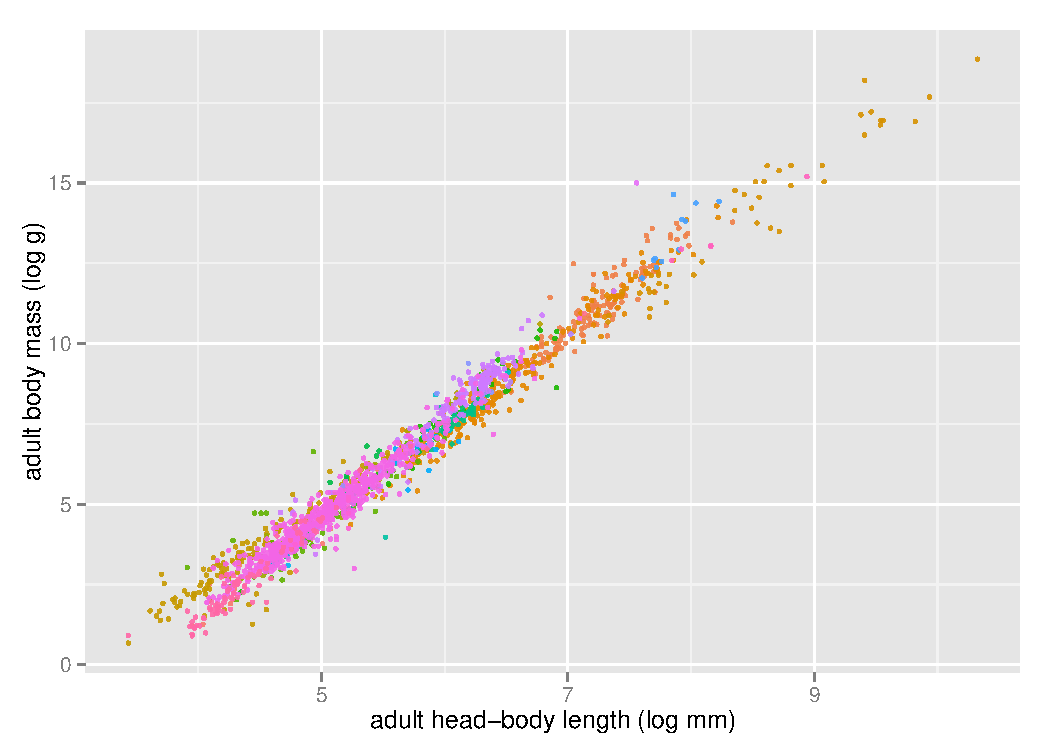
\includegraphics[width=\maxwidth]{figure/unnamed-chunk-21} 

\end{knitrout}

\end{frame}

\begin{frame}[fragile]
  \frametitle{Visualizing}
\begin{knitrout}\scriptsize
\definecolor{shadecolor}{rgb}{0.969, 0.969, 0.969}\color{fgcolor}\begin{kframe}
\begin{alltt}
gpan <- gpan + \hlfunctioncall{geom_point}(alpha = 0.9, size = 0.7,
                          mapping = \hlfunctioncall{aes}(colour = family))
gpan <- gpan + \hlfunctioncall{theme}(axis.text = \hlfunctioncall{element_text}(size = 6),
                     axis.title = \hlfunctioncall{element_text}(size = 8),
                     strip.text = \hlfunctioncall{element_text}(size = 6))
gpan <- gpan + \hlfunctioncall{facet_wrap}(~ order)
\end{alltt}
\end{kframe}
\end{knitrout}

\end{frame}

\begin{frame}[fragile]
  \frametitle{Visulizing}
\begin{knitrout}\scriptsize
\definecolor{shadecolor}{rgb}{0.969, 0.969, 0.969}\color{fgcolor}
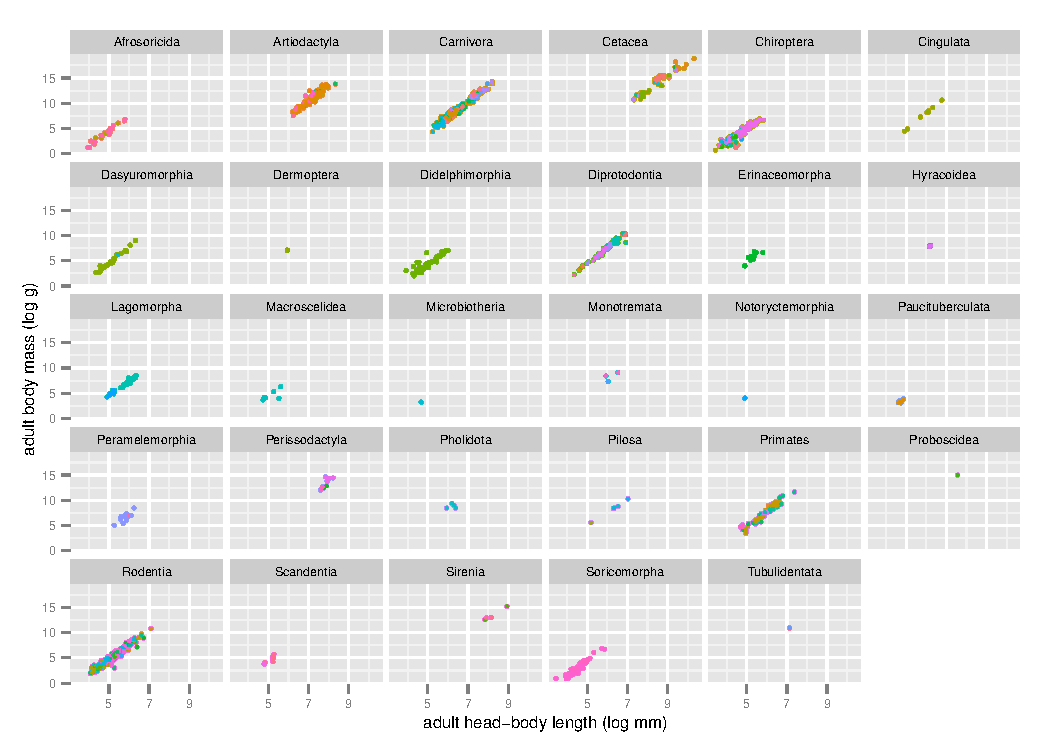
\includegraphics[width=\maxwidth]{figure/unnamed-chunk-23} 

\end{knitrout}

\end{frame}

\begin{frame}[fragile]
  \frametitle{Save our plot}

  If you aren't using knitr/Sweave (you should!), you can save your ggplot for use later.

\begin{knitrout}\scriptsize
\definecolor{shadecolor}{rgb}{0.969, 0.969, 0.969}\color{fgcolor}\begin{kframe}
\begin{alltt}
\hlfunctioncall{ggsave}(filename = \hlstring{'pantheria_facet.png'},
       plot = gpan)
\end{alltt}
\end{kframe}
\end{knitrout}


\end{frame}

\end{document}
